% ============================================================
%  MTH636 -- Game Theory | Lecture 1
%  The Beauty Contest Game & Strategic Thinking
%  Dr. Soumyarup Sadhukhan, IIT Kanpur
% ============================================================
\documentclass[12pt, a4paper]{article}

% ============================================================
%  MTH636 -- Game Theory
%  Notes Preamble — Color-Coded, TikZ-Enhanced
% ============================================================

% --- Core packages ---
\usepackage[T1]{fontenc}
\usepackage[utf8]{inputenc}
\usepackage{lmodern}
\usepackage[margin=2.5cm, top=2.8cm, bottom=2.8cm]{geometry}
\usepackage{microtype}

% --- Math ---
\usepackage{amsmath, amssymb, amsthm, mathtools}
\usepackage{bm}        % bold math
\usepackage{cancel}    % strike-through in math

% --- Color & Boxes ---
\usepackage[dvipsnames, svgnames, x11names, table]{xcolor}
\usepackage[most]{tcolorbox}
\tcbuselibrary{breakable, skins, theorems}

% --- TikZ & Diagrams ---
\usepackage{tikz}
\usepackage{tikz-qtree}
\usetikzlibrary{arrows.meta, positioning, shapes.geometric, fit, backgrounds,
                decorations.pathreplacing, calc, matrix, trees}
\usepackage{pgfplots}
\pgfplotsset{compat=1.18}

% --- Tables ---
\usepackage{booktabs}
\usepackage{multirow}
\usepackage{array}
\usepackage{tabularx}
\usepackage{makecell}

% --- Typography & Layout ---
\usepackage{enumitem}
\usepackage{parskip}
\usepackage{fancyhdr}
\usepackage{titlesec}
\usepackage{titletoc}
\usepackage{hyperref}
\usepackage{graphicx}
\usepackage{float}
\usepackage{caption}

% --- Color Palette ---
\definecolor{defblue}{HTML}{1A5276}      % Definition header
\definecolor{defbluebg}{HTML}{D6EAF8}    % Definition background
\definecolor{thmgreen}{HTML}{1E8449}     % Theorem header
\definecolor{thmbg}{HTML}{D5F5E3}        % Theorem background
\definecolor{exorange}{HTML}{B7770D}     % Example header
\definecolor{exbg}{HTML}{FEF9E7}         % Example background
\definecolor{warnred}{HTML}{922B21}      % Warning/Key Insight header
\definecolor{warnbg}{HTML}{FADBD8}       % Warning background
\definecolor{noticegray}{HTML}{2C3E50}   % Note header
\definecolor{noticebg}{HTML}{EBF5FB}     % Note background
\definecolor{taketawayyellow}{HTML}{7D6608} % Key Takeaway header
\definecolor{takeawaybg}{HTML}{FDFEFE}   % Takeaway background
\definecolor{accentpurple}{HTML}{6C3483} % Accent / proof
\definecolor{lightgray}{HTML}{F2F3F4}    % shading

% ============================================================
%  TCOLORBOX ENVIRONMENTS
% ============================================================

% -- Definition (Blue) --
\newtcolorbox{defbox}[2][]{
  enhanced, breakable,
  colback=defbluebg, colframe=defblue, coltitle=white,
  fonttitle=\bfseries\sffamily,
  title={Definition: #2},
  attach boxed title to top left={yshift=-2mm, xshift=4mm},
  boxed title style={colback=defblue, rounded corners},
  arc=4pt, boxrule=1.2pt,
  left=6pt, right=6pt, top=8pt, bottom=6pt,
  #1
}

% -- Theorem / Proposition (Green) --
\newtcolorbox{thmbox}[2][]{
  enhanced, breakable,
  colback=thmbg, colframe=thmgreen, coltitle=white,
  fonttitle=\bfseries\sffamily,
  title={Theorem: #2},
  attach boxed title to top left={yshift=-2mm, xshift=4mm},
  boxed title style={colback=thmgreen, rounded corners},
  arc=4pt, boxrule=1.2pt,
  left=6pt, right=6pt, top=8pt, bottom=6pt,
  #1
}

% -- Proposition (Green variant) --
\newtcolorbox{propbox}[2][]{
  enhanced, breakable,
  colback=thmbg, colframe=thmgreen!70!black, coltitle=white,
  fonttitle=\bfseries\sffamily,
  title={Proposition: #2},
  attach boxed title to top left={yshift=-2mm, xshift=4mm},
  boxed title style={colback=thmgreen!70!black, rounded corners},
  arc=4pt, boxrule=1.2pt,
  left=6pt, right=6pt, top=8pt, bottom=6pt,
  #1
}

% -- Example (Orange/Yellow) --
\newtcolorbox{exbox}[2][]{
  enhanced, breakable,
  colback=exbg, colframe=exorange, coltitle=white,
  fonttitle=\bfseries\sffamily,
  title={Example: #2},
  attach boxed title to top left={yshift=-2mm, xshift=4mm},
  boxed title style={colback=exorange, rounded corners},
  arc=4pt, boxrule=1.2pt,
  left=6pt, right=6pt, top=8pt, bottom=6pt,
  #1
}

% -- Key Insight / Warning (Red) --
\newtcolorbox{warnbox}[2][]{
  enhanced, breakable,
  colback=warnbg, colframe=warnred, coltitle=white,
  fonttitle=\bfseries\sffamily,
  title={Key Insight: #2},
  attach boxed title to top left={yshift=-2mm, xshift=4mm},
  boxed title style={colback=warnred, rounded corners},
  arc=4pt, boxrule=1.2pt,
  left=6pt, right=6pt, top=8pt, bottom=6pt,
  #1
}

% -- Note (Gray-Blue) --
\newtcolorbox{notebox}[1][]{
  enhanced, breakable,
  colback=noticebg, colframe=noticegray!60, coltitle=white,
  fonttitle=\bfseries\sffamily,
  title={Note},
  attach boxed title to top left={yshift=-2mm, xshift=4mm},
  boxed title style={colback=noticegray!60, rounded corners},
  arc=4pt, boxrule=0.8pt,
  left=6pt, right=6pt, top=8pt, bottom=6pt,
  #1
}

% -- Key Takeaway --
\newtcolorbox{takebox}[1][]{
  enhanced, breakable,
  colback=takeawaybg, colframe=taketawayyellow, coltitle=white,
  fonttitle=\bfseries\sffamily,
  title={Key Takeaway},
  attach boxed title to top left={yshift=-2mm, xshift=4mm},
  boxed title style={colback=taketawayyellow, rounded corners},
  arc=4pt, boxrule=1.2pt,
  left=6pt, right=6pt, top=8pt, bottom=6pt,
  #1
}

% -- Intuition --
\newtcolorbox{intubox}[1][]{
  enhanced, breakable,
  colback=accentpurple!8, colframe=accentpurple!60, coltitle=white,
  fonttitle=\bfseries\sffamily,
  title={Intuition},
  attach boxed title to top left={yshift=-2mm, xshift=4mm},
  boxed title style={colback=accentpurple!80, rounded corners},
  arc=4pt, boxrule=0.8pt,
  left=6pt, right=6pt, top=8pt, bottom=6pt,
  #1
}

% ============================================================
%  PAYOFF MATRIX HELPER
%  Usage: inside tabular, use \payoff{a}{b} for (a,b)
% ============================================================
\newcommand{\payoff}[2]{$(#1,\;#2)$}
\newcommand{\nash}[2]{\underline{$#1$},\underline{$#2$}}  % underline NE payoffs
\newcommand{\Nset}{\mathbb{N}}
\newcommand{\Rset}{\mathbb{R}}
\newcommand{\Sset}{\mathcal{S}}
\newcommand{\Ui}{u_i}

% ============================================================
%  SECTION FORMATTING
% ============================================================
\titleformat{\section}
  {\large\bfseries\sffamily\color{defblue}}
  {\thesection}{1em}{}[\titlerule]

\titleformat{\subsection}
  {\normalsize\bfseries\sffamily\color{thmgreen!80!black}}
  {\thesubsection}{1em}{}

\titleformat{\subsubsection}
  {\normalsize\itshape\sffamily\color{exorange!80!black}}
  {\thesubsubsection}{1em}{}

% ============================================================
%  HEADER / FOOTER
% ============================================================
\pagestyle{fancy}
\fancyhf{}
\fancyhead[L]{\sffamily\small\color{defblue} MTH636 -- Game Theory}
\fancyhead[R]{\sffamily\small\color{defblue} \leftmark}
\fancyfoot[C]{\sffamily\small\thepage}
\renewcommand{\headrulewidth}{0.4pt}

% ============================================================
%  HYPERREF SETUP
% ============================================================
\hypersetup{
  colorlinks=true,
  linkcolor=defblue,
  urlcolor=thmgreen,
  citecolor=accentpurple,
  bookmarksnumbered=true,
  pdftitle={MTH636 Game Theory Notes},
  pdfauthor={MTH636 Student Notes}
}

% ============================================================
%  MISC HELPERS
% ============================================================
\newcommand{\BR}{\text{BR}}        % Best Response
\newcommand{\NE}{\text{NE}}        % Nash Equilibrium
\newcommand{\SPNE}{\text{SPNE}}    % Subgame Perfect NE
\newcommand{\Dom}{\text{dom}}      % Dominance
\newcommand{\mixs}[1]{\sigma_{#1}} % Mixed strategy
\newcommand{\pures}[1]{s_{#1}}     % Pure strategy


% ============================================================
\begin{document}

% Title
\begin{center}
  {\LARGE\bfseries\sffamily\color{defblue} MTH636 -- Game Theory}\\[6pt]
  {\Large\sffamily Lecture 1: Strategic Thinking \& the Beauty Contest Game}\\[4pt]
  {\normalsize\sffamily Dr.\ Soumyarup Sadhukhan \quad | \quad Dept.\ of Statistics \& Data Science, IIT Kanpur}
\end{center}
\vspace{0.5cm}
\hrule height 1.5pt
\vspace{0.3cm}

\tableofcontents
\newpage

% ============================================================
\section{Motivation: What Is Game Theory?}

Game theory is the mathematical study of \textbf{strategic interaction} -- situations where the outcome for each participant depends not only on their own actions, but also on the actions of others.

\begin{intubox}
  \textbf{Optimization vs.\ Strategy.}
  In a standard optimization problem (e.g., calculus, operations research), you maximize/minimize a function that depends only on your own choices. In a \emph{strategic} problem, your payoff depends on what \emph{everyone else} does -- so you must think about what others will do, which depends on what they think \emph{you} will do, and so on. This feedback loop is the heart of game theory.
\end{intubox}

% ============================================================
\section{The Beauty Contest Game (Keynes' Guessing Game)}

\subsection{Setup}

\begin{defbox}{The $p$-Beauty Contest Game}
  \begin{itemize}[leftmargin=*, label=\textbullet]
    \item $n$ players, each independently chooses a real number $x_i \in [0, 100]$.
    \item After all choices are made, compute the \textbf{average}:
      \[
        \bar{x} = \frac{1}{n} \sum_{i=1}^{n} x_i
      \]
    \item The \textbf{target} is:
      \[
        T(\mathbf{x}) = \frac{2}{3}\,\bar{x}
      \]
    \item The \textbf{winner} is the player whose choice $x_i$ is closest to $T(\mathbf{x}) = \frac{2}{3}\bar{x}$.
    \item (In the generalized version: target $= p\bar{x}$ for parameter $p \in (0,\infty)$.)
  \end{itemize}
\end{defbox}

\begin{notebox}
  This is a \emph{simultaneous} game -- no player sees others' choices before deciding. It is \emph{not} a pure optimization problem because the target itself depends on everyone's choices.
\end{notebox}

% ============================================================
\subsection{Levels of Reasoning}

To find a good strategy, players must think about what others will do. This leads to \textbf{iterated reasoning}:

\begin{center}
\renewcommand{\arraystretch}{1.4}
\begin{tabular}{>{\bfseries\sffamily\color{defblue}}c c c}
  \toprule
  \rowcolor{defbluebg}
  Level & Belief About Others & Choice \\
  \midrule
  Level 0 & No strategic adjustment (random/naive) & $\approx 50$ \\
  Level 1 & Others are Level 0 (avg $\approx 50$) & $\frac{2}{3} \times 50 \approx 33$ \\
  Level 2 & Others are Level 1 (avg $\approx 33$) & $\frac{2}{3} \times 33 \approx 22$ \\
  Level 3 & Others are Level 2 (avg $\approx 22$) & $\frac{2}{3} \times 22 \approx 15$ \\
  $\vdots$ & $\vdots$ & $\vdots$ \\
  $\infty$ & Infinite mutual reasoning & $0$ \\
  \bottomrule
\end{tabular}
\end{center}

\medskip
The chain of reasoning:
\[
  50 \;\longrightarrow\; 33 \;\longrightarrow\; 22 \;\longrightarrow\; 15 \;\longrightarrow\; 10 \;\longrightarrow\; 7 \;\longrightarrow\; \cdots \;\longrightarrow\; 0
\]

\begin{center}
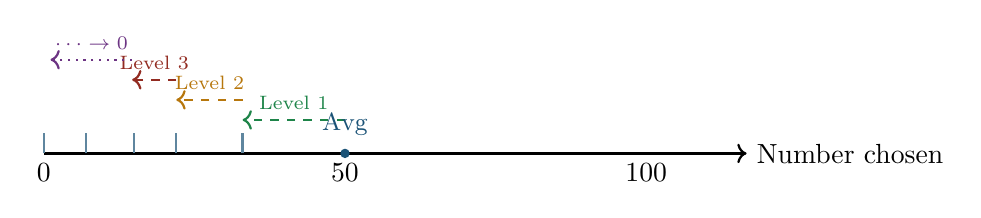
\begin{tikzpicture}[scale=0.85]
  \draw[->, thick] (0,0) -- (10.5,0) node[right] {Number chosen};
  \foreach \x/\label in {0/0, 3.3/33, 2.2/22, 1.5/15, 0.7/7} {
    \draw[thick, defblue!70] (\x*0.9,0) -- (\x*0.9,0.3);
  }
  \node[below] at (0,0) {$0$};
  \node[below] at (4.5,0) {$50$};
  \node[below] at (9,0) {$100$};
  \draw[dashed, thmgreen, thick, ->] (4.5,0.5) -- (2.97,0.5) node[midway, above, font=\scriptsize] {Level 1};
  \draw[dashed, exorange, thick, ->] (2.97,0.8) -- (1.98,0.8) node[midway, above, font=\scriptsize] {Level 2};
  \draw[dashed, warnred, thick, ->] (1.98,1.1) -- (1.32,1.1) node[midway, above, font=\scriptsize] {Level 3};
  \draw[dotted, accentpurple, thick, ->] (1.32,1.4) -- (0.1,1.4) node[midway, above, font=\scriptsize] {$\cdots \to 0$};
  \fill[defblue] (4.5,0) circle (2pt) node[above=3pt, font=\small] {Avg};
\end{tikzpicture}
\end{center}

% ============================================================
\subsection{A Dominance-Style Argument}

This section makes the convergence to 0 \emph{rigorous} using a \textbf{dominance argument}, not just intuition.

\begin{propbox}{No rational player chooses above $\frac{200}{3} \approx 66.67$}
  \textbf{Argument:} Since all $x_i \in [0,100]$, we have $\bar{x} \leq 100$. Therefore:
  \[
    T(\mathbf{x}) = \frac{2}{3}\bar{x} \leq \frac{2}{3} \times 100 = 66.\overline{6}
  \]
  So no matter what others do, the target is \emph{never} above $66.\overline{6}$. Any choice $x_i > 66.\overline{6}$ is always farther from the target than $x_i = 66.\overline{6}$. Hence choosing above $66.\overline{6}$ is \textbf{dominated} -- a rational player eliminates it.
\end{propbox}

\subsubsection{Iterating the Argument (IESDS)}

Once all rational players restrict to $[0, 66.\overline{6}]$, we can apply the argument again:

\begin{align*}
  [0, 100] &\xrightarrow{\text{Round 1}} \left[0,\; \tfrac{2}{3} \times 100\right] = [0,\; 66.\overline{6}] \\
           &\xrightarrow{\text{Round 2}} \left[0,\; \tfrac{2}{3} \times 66.\overline{6}\right] = [0,\; 44.\overline{4}] \\
           &\xrightarrow{\text{Round 3}} \left[0,\; \tfrac{2}{3} \times 44.\overline{4}\right] = [0,\; 29.63] \\
           &\xrightarrow{\text{Round } k} \left[0,\; 100 \cdot \left(\tfrac{2}{3}\right)^k\right] \\
           &\xrightarrow{k \to \infty} \{0\}
\end{align*}

After infinitely many rounds, \emph{only 0 survives}. This process is called \textbf{Iterated Elimination of Strictly Dominated Strategies (IESDS)}.

\begin{center}
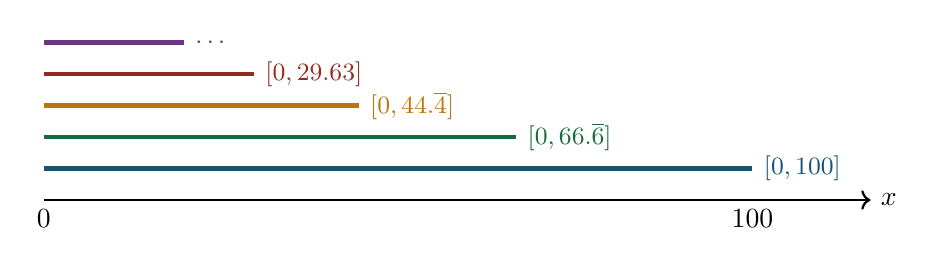
\begin{tikzpicture}[scale=1]
  \draw[->, thick] (0,0) -- (10.5,0) node[right] {$x$};
  \draw[defblue, ultra thick] (0,0.4) -- (9,0.4) node[right, font=\small] {$[0,100]$};
  \draw[thmgreen!80!black, ultra thick] (0,0.8) -- (6,0.8) node[right, font=\small] {$[0,66.\overline{6}]$};
  \draw[exorange, ultra thick] (0,1.2) -- (4,1.2) node[right, font=\small] {$[0,44.\overline{4}]$};
  \draw[warnred, ultra thick] (0,1.6) -- (2.67,1.6) node[right, font=\small] {$[0,29.63]$};
  \draw[accentpurple, ultra thick] (0,2.0) -- (1.78,2.0) node[right, font=\small] {$\cdots$};
  \node[below] at (0,0) {$0$};
  \node[below] at (9,0) {$100$};
\end{tikzpicture}
\end{center}

% ============================================================
\subsection{What Assumptions Are Used?}

\begin{warnbox}{The Two Critical Assumptions}
  The conclusion ``all players choose 0'' relies on \emph{two} distinct assumptions:
  \begin{enumerate}[label=\textbf{A\arabic*.}, leftmargin=*]
    \item \textbf{Rationality}: Each player avoids dominated strategies.
    \item \textbf{Common Knowledge of Rationality (CKR)}: \emph{I am rational. I know you are rational. I know that you know that I am rational. I know that you know that I know \ldots} and so on, to all orders.
  \end{enumerate}
  \emph{Rationality alone is insufficient} -- you need CKR to justify each round of elimination.
\end{warnbox}

\begin{notebox}
  In real-world experiments with first-time players, the winning number is typically \textbf{much larger than 0} (often around 20--35). This is not a failure of the theory -- it reveals that real people apply only 1--3 levels of reasoning, and CKR does not hold in practice.
\end{notebox}

% ============================================================
\section{The Keynesian Beauty Contest Analogy}

John Maynard Keynes drew a famous analogy between financial markets and newspaper beauty contests:

\begin{exbox}{Keynes' Analogy (1936)}
  In 1930s newspaper contests, readers voted on which face was prettiest from a set of photographs. The prize went to whoever correctly predicted the \emph{average opinion} -- not who actually had the prettiest face.

  \smallskip
  Keynes argued financial speculation works similarly:
  \begin{itemize}[leftmargin=*, label=--]
    \item It is not about picking the stock that \emph{you} think is best.
    \item It is about predicting what \emph{the market} will think is best.
    \item Or even better: predicting what the market thinks the market will think is best.
    \item This leads to recursive, self-referential reasoning.
  \end{itemize}
\end{exbox}

% ============================================================
\section{Generalization: The $p$-Beauty Contest}

\begin{defbox}{Generalized $p$-Beauty Contest}
  Replace $\frac{2}{3}$ by a parameter $p \in (0,\infty)$.
  Players choose $x_i \in [0,100]$ and the target is $T_p(\mathbf{x}) = p\bar{x}$.
\end{defbox}

\medskip
\begin{center}
\renewcommand{\arraystretch}{1.4}
\begin{tabular}{>{\bfseries}c p{7cm}}
  \toprule
  \rowcolor{defbluebg}
  Case & Prediction \\
  \midrule
  $0 < p < 1$ & \textbf{Unique equilibrium}: all choose $x_i = 0$. IESDS converges to 0. \\
  \rowcolor{exbg}
  $p = 1$ & \textbf{Every common choice} is an equilibrium (if all choose the same $c$, target is $c$). \\
  $p > 1$ & Reasoning moves \emph{upward}. Boundary effects at 100. \\
  \bottomrule
\end{tabular}
\end{center}

% ============================================================
\section{Sequential Version}

\begin{exbox}{Sequential Beauty Contest}
  Now suppose three players move \textbf{in order}:
  \begin{enumerate}[label=\textbf{Step \arabic*.}]
    \item Player 1 chooses $x$.
    \item Player 2 observes $x$ and chooses $y$.
    \item Player 3 observes $(x,y)$ and chooses $z$.
  \end{enumerate}
  The target is still $\dfrac{2}{3} \cdot \dfrac{x+y+z}{3}$.

  \medskip
  \textbf{Key question:} Does observing others' choices change the outcome? Does the equilibrium still predict 0?

  \medskip
  (This preview leads into the study of \textbf{extensive-form games} and \textbf{backward induction}, covered in later lectures.)
\end{exbox}

% ============================================================
\section{Summary \& Key Takeaways}

\begin{takebox}
  \begin{enumerate}[label=\textbf{\arabic*.}, leftmargin=*]
    \item Game theory studies \textbf{strategic settings} where each player's payoff depends on others' actions -- not just optimization.
    \item The beauty contest game illustrates that rational behavior requires not just rationality, but \textbf{common knowledge of rationality (CKR)}.
    \item The solution concept used here is \textbf{IESDS} (Iterated Elimination of Strictly Dominated Strategies): repeatedly remove strategies that are always worse than some other strategy.
    \item IESDS under CKR predicts choosing $0$, yet experiments show most people choose between 20--35 -- indicating limited levels of strategic reasoning in practice.
    \item Keynes' analogy: financial markets involve not just valuation of assets, but \emph{predicting others' predictions} -- a recursive, game-theoretic process.
  \end{enumerate}
\end{takebox}

% ============================================================
\section*{References}

\begin{itemize}[leftmargin=*, label={[}]
  \item[\lbrack 1\rbrack] Keynes, J.\ M.\ (1936). \textit{The General Theory of Employment, Interest and Money}. Macmillan.
  \item[\lbrack 2\rbrack] Nagel, R.\ (1995). ``Unraveling in Guessing Games: An Experimental Study.'' \textit{American Economic Review}, 85(5), 1313--1326.
  \item[\lbrack 3\rbrack] Duffy, J.\ and Nagel, R.\ (1997). ``On the Robustness of Behavior in Experimental Beauty Contest Games.'' \textit{Economic Journal}, 107(445), 1684--1700.
  \item[\lbrack 4\rbrack] Camerer, C.\ F., Ho, T.-H., and Chong, J.-K.\ (2004). ``A Cognitive Hierarchy Model of Games.'' \textit{Quarterly Journal of Economics}, 119(3), 861--898.
\end{itemize}

\end{document}